% Chapter Template

\chapter{Conclusion} % Main chapter title

\label{Chapter6} % Change X to a consecutive number; for referencing this chapter elsewhere, use \ref{ChapterX}

\lhead{Chapter 6. \emph{Conclusion}} % Change X to a consecutive number; this is for the header on each page - perhaps a shortened title

%----------------------------------------------------------------------------------------
%	SECTION 1
%----------------------------------------------------------------------------------------

\section{Recommendation for Future Research}

In the past few years, Graph Neural Networks (GNNs) have gained a lot of popularity. Traditional Deep Learning based models like CNNs and RNNs work on data like Images and Text, which can be regarded as Euclidean data. GNNs extend the power of these models to graph data which is non-Euclidean in nature. Molecular structure of proteins and people in a social graph can be considered as examples of non-Euclidean data. GNNs have also achieved great success in tasks on similar datasets in the recent years\cite{Wu2020GraphCN,fout2017protein}. This has made GNNs an active research topic in Artificial Intelligence today leading to new and improved graph based models like Graph Convolutional Network (GCN)\cite{kipf2017semi} and Graph Attention Network\cite{velickovic2018graph}.

% Since the Luxury-Standard data can also be modelled as a Social Graph, there is reason to believe Graph Neural Networks may perform well on this data.

The Luxury-Standard dataset contains information about both - the emails sent by the employees and the mail content. This means that the current data can be modelled as a social network graph after which a GNN can be applied to it. The advantage of GNNs is that they are able to leverage information from the neighbour nodes in the social graph similar to how a CNN exploits the spatial data in an image by looking at the adjacent pixels when sliding a window over the input. 

The data can be represented as a graph by converting each employee and mail as a node in a heterogeneous graph. For each $e_t : s \rightarrow r$, an edge is constructed between $s$-$e_t$ and $r$-$e_t$. A design choice over here can give rise to two different kind of graphs - one containing an edge between $s$-$r$ and another one without any $s$-$r$ edge. 

\clearpage

\begin{figure}[!tbp]
  \centering
\subfloat[Without Sender-Receiver Edge]{    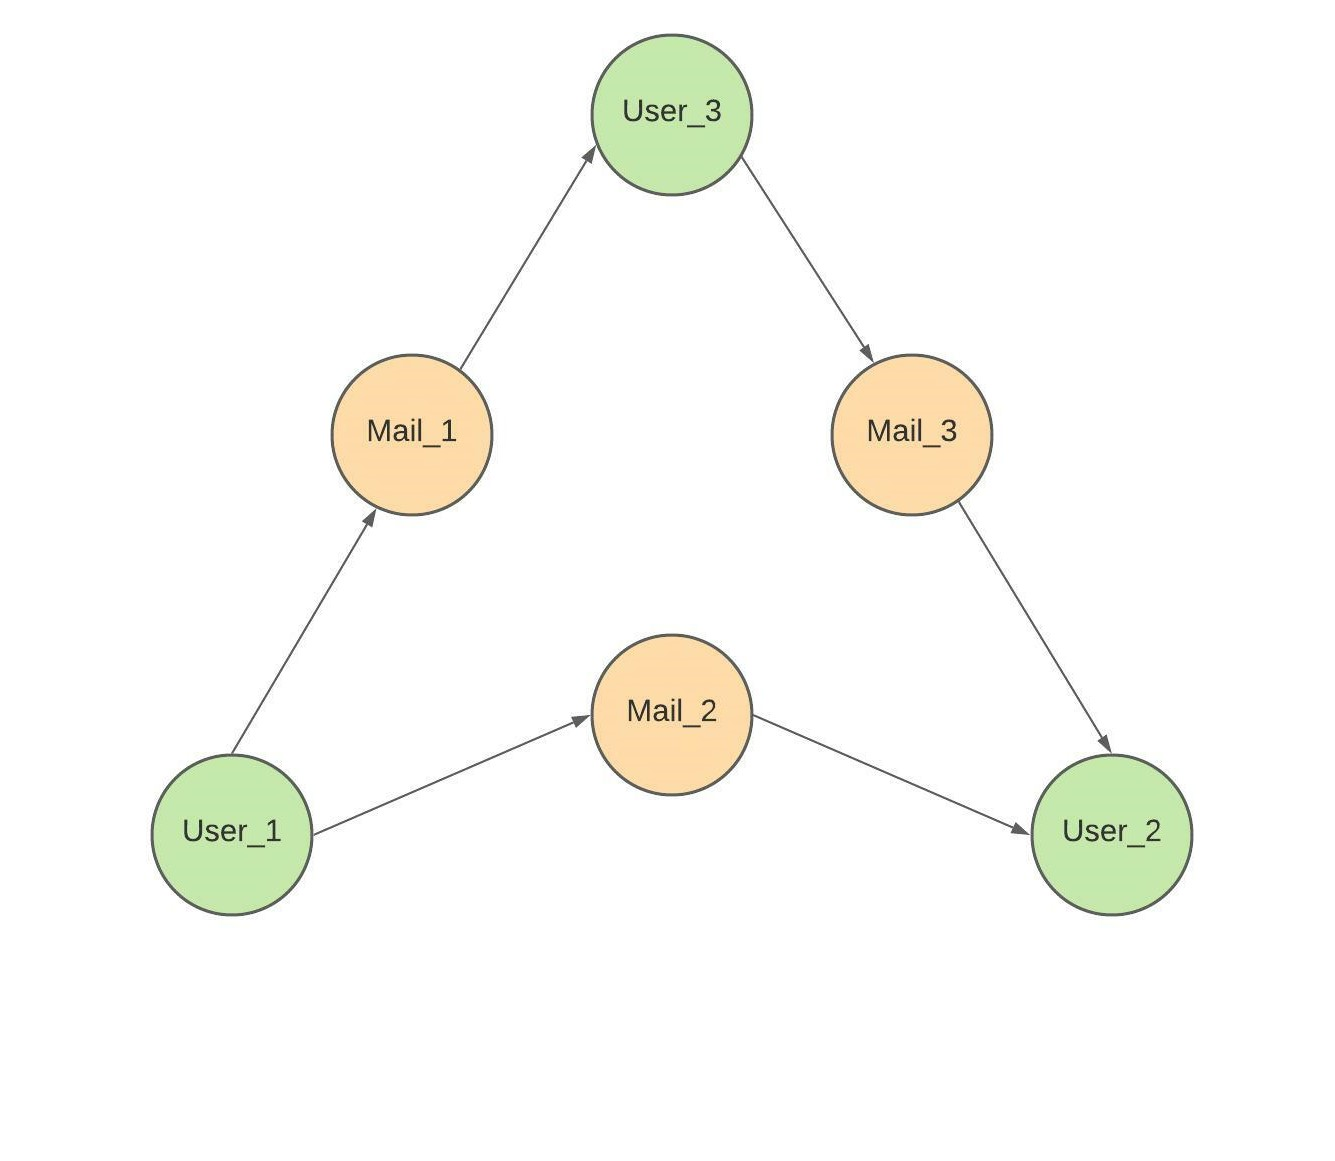
\includegraphics[width=0.48\textwidth]{Figures/graph_type_1.jpeg}} 
\subfloat[With Sender-Receiver Edge]{    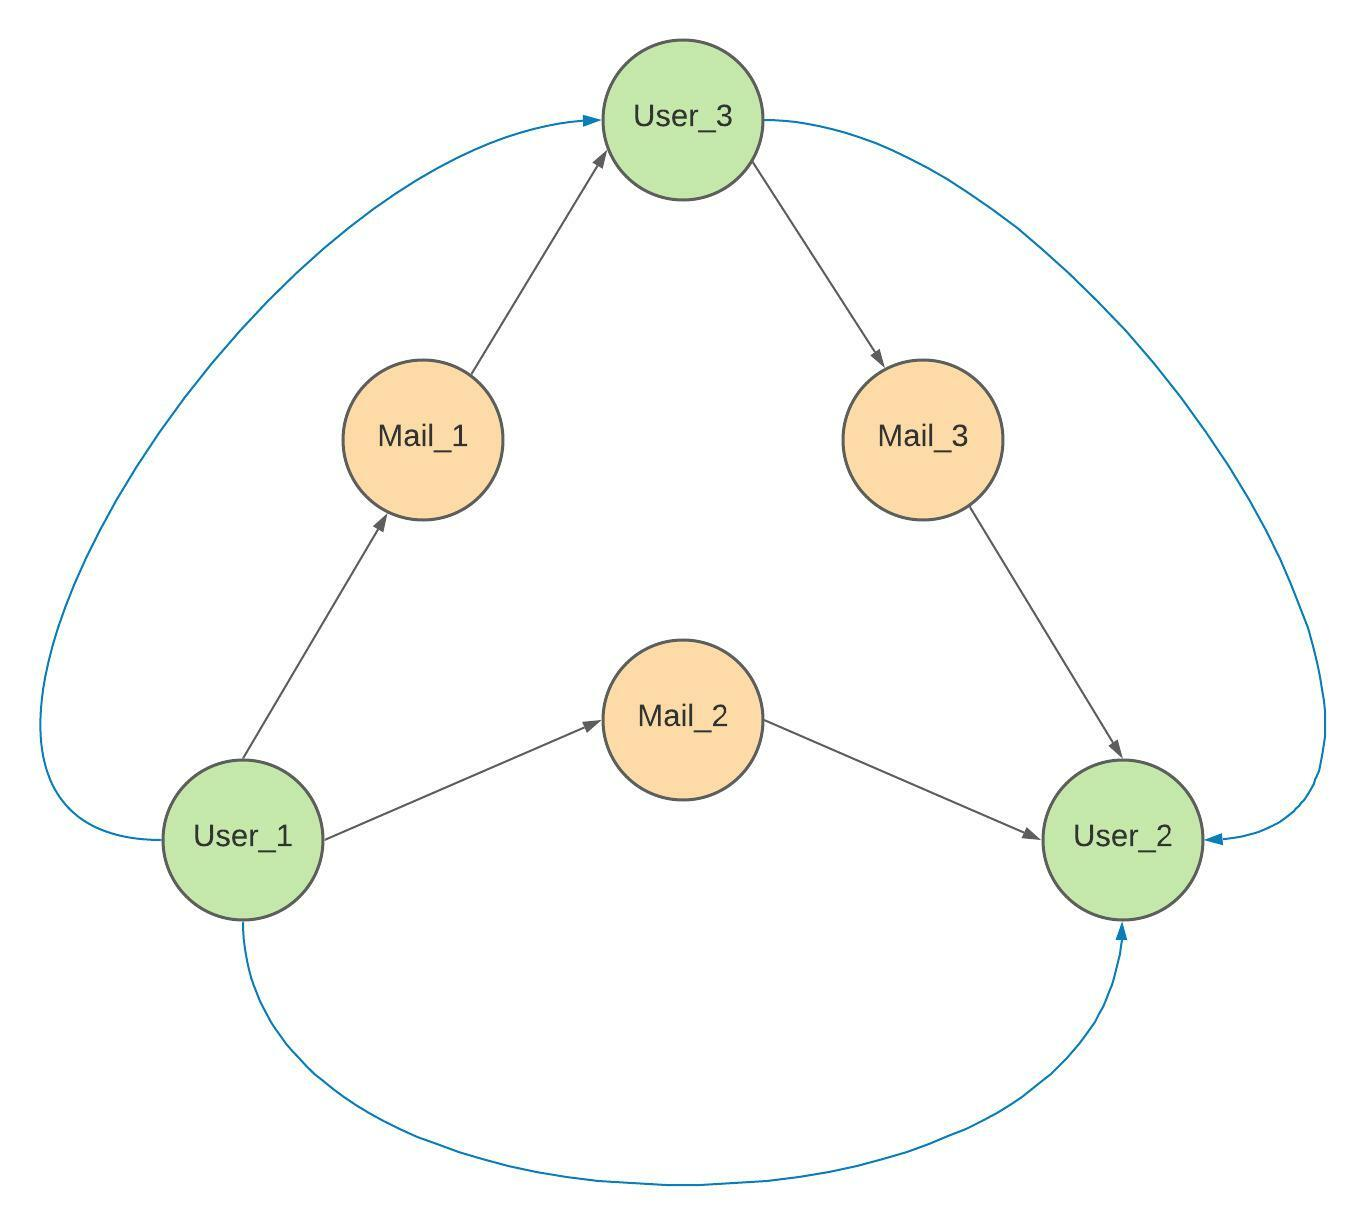
\includegraphics[width=0.48\textwidth]{Figures/graph_type_2.jpeg}}
    \caption{Data as Heterogeneous Graph}
  \label{fig:data_as_graph}
\end{figure}


Figure~\ref{fig:data_as_graph} shows an example of how the graph would look if created using either of the above mentioned methods. Once the data is in a compatible format, graph based machine learning libraries like PyTorch-Geometric\cite{Fey/Lenssen/2019} and StellarGraph\cite{StellarGraph} can be used to apply State-of-the-Art graph based methods on it.

\section{Conclusion}

Predicting the probability of getting a reply to a corporate mail would help the employees plan better. It can also help them write emails which are more likely to get a reply. The email body contains a lot of information that could help predict the chances of getting a reply back. But looking beyond this, we can see that there are many more factors involved like preferences of the sender and receiver, their workplace relations with each other, style of the message, and so on.

Incorporating these various features along with the email body cannot be done in a simple Transformer model like BERT which works solely on textual input. The proposed MultiModal architecture addresses this issue by using BERT to generate embeddings for the email body which is then concatenated with other numerical and categorical features to form the final email representation. These changes improve the accuracy by more than $\sim$4\% as compared to purely text based methods like BERT and RoBERTa.